\section{RNA-Seq: alignment}
To make more sense of the RNA-Seq data, we try to locate the detected sequences back in a reference genome (this is often called mapping and aligning).
The reference genome should represent the most common sequence of the chromosomes of the human population.
Please read the first paragraph (3 sentences) of the following url: \url{http://en.wikipedia.org/wiki/Reference_genome}
\begin{itemize}
	\item On how many individuals is hg19 based?
\end{itemize}
For RNA-Seq we need specialized RNA aligners, able to cope with gaps that originate from splicing.
There are quite some of these aligners around. We will make use the tool ``\textit{\underline{RNA STAR} Gapped-read mapper for RNA-seq data}''.
Load the aligner, select the following settings and leave the rest on default, and run an alignment for \textit{miR-23b (clean)} and \textit{control sample (clean)}. \textbf{Alignment is a computational very very heavy task so do NOT re-run it if you don't have a good reason, or you will have to give a treat.}\\
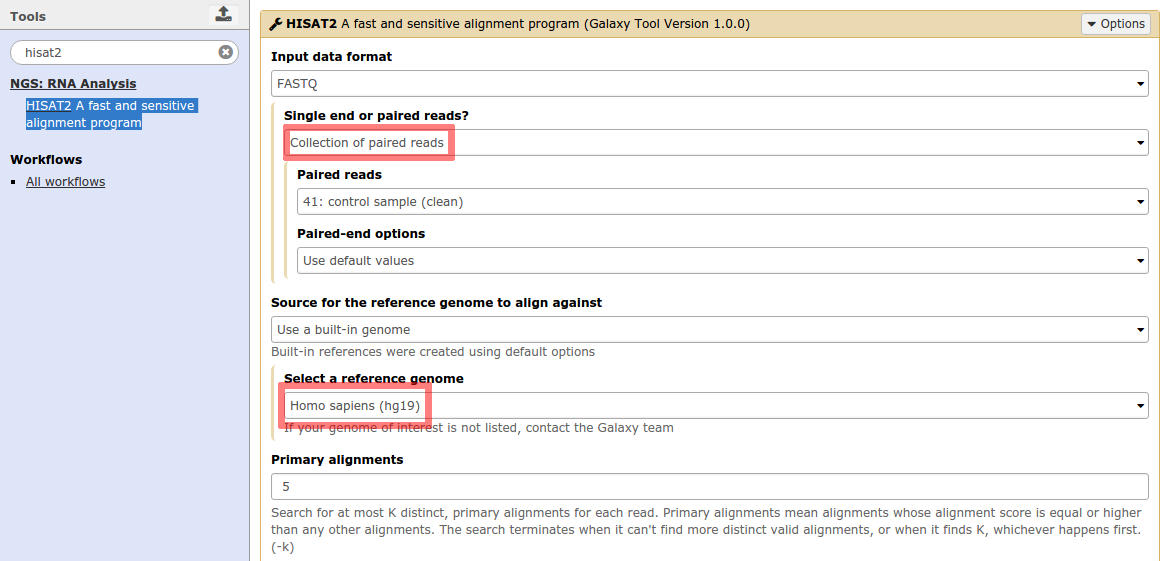
\includegraphics[width=\textwidth]{figures/alignment_01.png}\\
Please rename the \textit{RNA STAR on ...: starmapped.bam} to ``\textit{RNA STAR on miR-23b: starmapped.bam}'' and ``\textit{RNA STAR on control sample: starmapped.bam}'' or something else that makes it easy to recognize.
If the alignments do not have their \textbf{database} (also referred to as \textbf{dbkey}) set, change it to hg19 as follows:\\
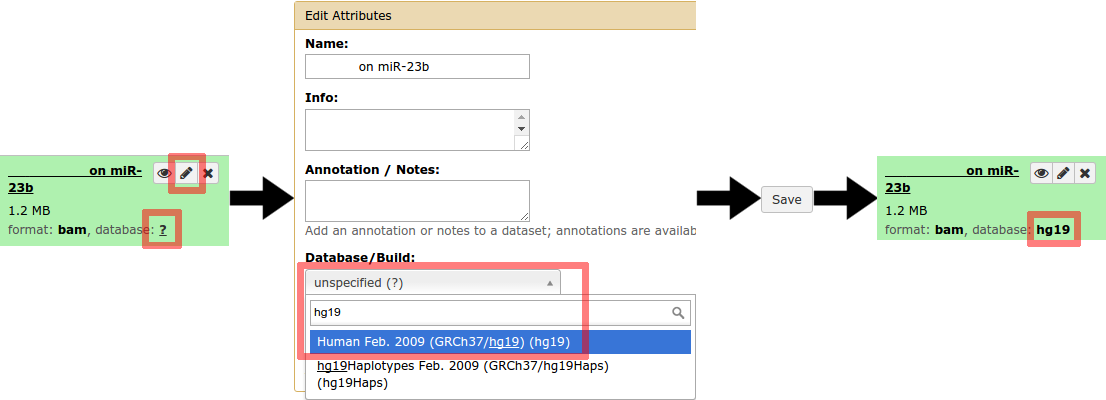
\includegraphics[width=\textwidth]{figures/alignment_02.png}\\
To get some general alignment statistics, run the tool ``\textit{\underline{Flagstat} tabulate descriptive stats for BAM datset}'' on \textit{miR-23b}.
\begin{itemize}
	\item How many reads are multi-mapping?
\end{itemize}
For now we have only seen FASTQ and summary files. To get an idea of what has been measured during the experiment, we can visualise the alignment. So, in the alignnment step we have been looking in hg19 where these sequences originate from, and this information is stored in the bam files. Import from the Shared Data library (\datalibrarydirrnaseqadvanced) the file ``\textit{ucsc\_refseq.gtf}'' into your history. Start the built-in visualization Trackster at one of the alignments (make sure the database is set to \textbf{hg19}):\\
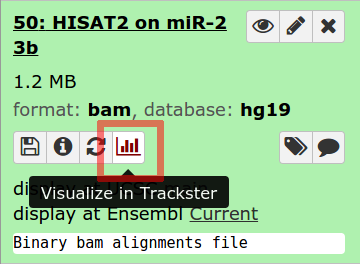
\includegraphics[scale=0.55]{figures/alignment_03}\\
Give it a name, press \textit{Create} and you will see a yellow bar, indicating that the bam file is being prepared. This means that the bam file is being converted into a file format that the browser is able to visualize.\\
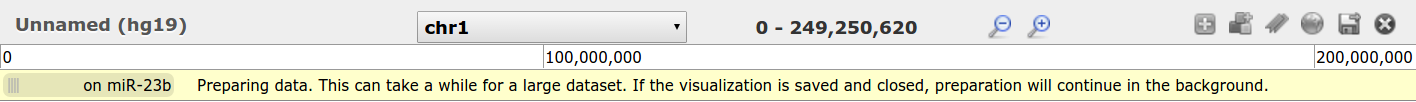
\includegraphics[width=\textwidth]{figures/alignment_04.png}\\
When this job is done, and it contains no error messages in the bars, which should look like the figure below, save it:\\
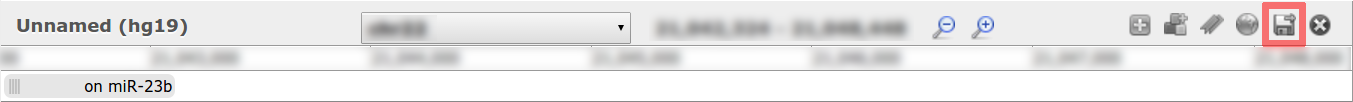
\includegraphics[width=\textwidth]{figures/alignment_05.png}\\
To add the other alignment, press the \textbf{[+]}-button:\\
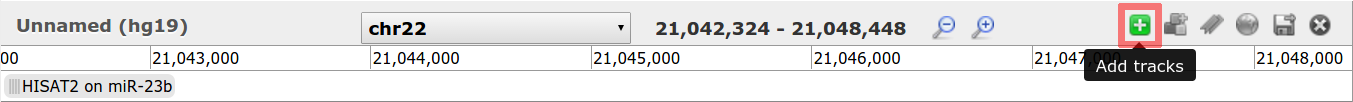
\includegraphics[width=\textwidth]{figures/alignment_06.png}\\
Now select the other alignment and press \textit{Add} and save it again:\\
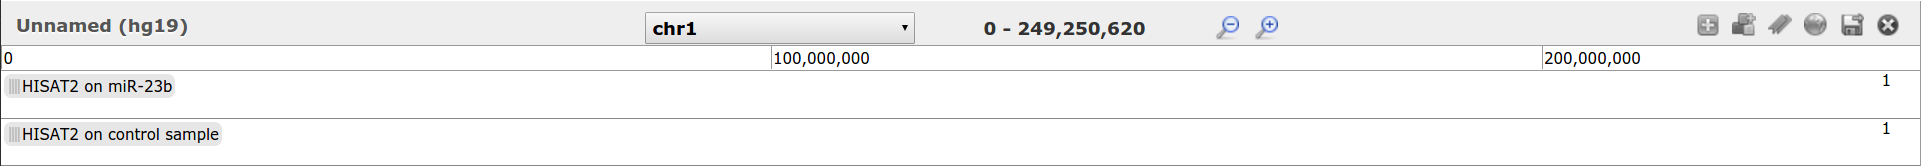
\includegraphics[width=\textwidth]{figures/alignment_07.png}\\
Remark that this is truncated data and you are supposed to see barely anything in here. Go to \textit{chr16}, to region \verb|chr16:15696870-15745667|.
\begin{itemize}
	\item Can you see where the introns and exons are located?
\end{itemize}
To help you answer this question, you can add ``\textit{ucsc\_refseq.gtf}'' that will visualize the exons and gene structure of a refseq gene annotation. It will only be visible if its database of the history item is set to hg19. Again, ensure this visualization is saved:\\
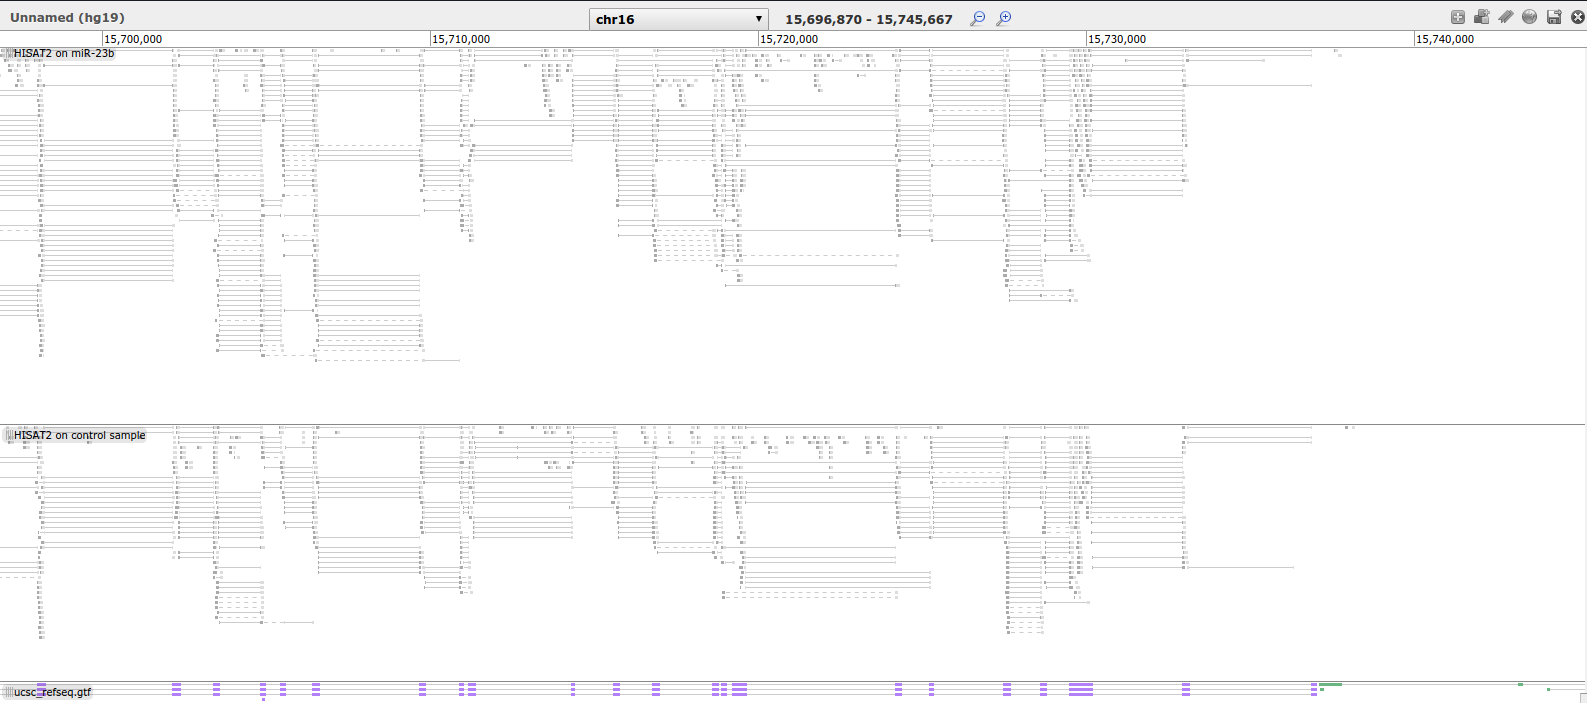
\includegraphics[width=\textwidth]{figures/alignment_08.png}\\
\begin{itemize}
	\item Can you go to \verb|chr15:60688011-60688099|, and explain what is going on there?
\end{itemize}
In the last question you can clearly see that you can observe biological facts from alignments where you couldn't extract this from the plain fastq files.
Because looking through all alignments 'by hand' is way too much work and prone to errors, we use these bam files for a variety of computer programs to estimate metrics for you instead.
These metrics can be insert size, expression levels, indel ratio's, etc., that may be used to test different hypotheses.

%The insert size is the size between the mate pairs in the alignment. Since the fragments (original part of RNA) are size selected, this should also be reflect in the alignment. Leave Trackster and run the Picard tool: ``Insertion size metrics for pairedd data''.

% @ todo
%- Ask question about insert size
